\documentclass{article}
\usepackage[T1]{fontenc}
\usepackage{lmodern}
\usepackage{graphicx}
\usepackage{amsmath,amssymb}
\usepackage[a4paper,margin=2cm]{geometry}
\usepackage[absolute,overlay]{textpos}
\setlength{\TPHorizModule}{1mm}
\setlength{\TPVertModule}{1mm}
\usepackage[indonesian]{babel}
\usepackage{hyperref}
\setlength{\emergencystretch}{2em}
% unit: Halaman 17

\begin{document}

% === Halaman 17 (llm) ===

\vspace{100.68mm}

Contoh elemen state dalam notasi HEX:
\vspace{10mm}

% deskripsi: Tabel yang berisi elemen state dalam notasi heksadesimal (HEX) dengan ukuran 4x4.
% bbox normalisasi: [0.2460, 0.3270, 0.5350, 0.6660]
\begin{textblock*}{60.69mm}(51.66mm,97.12mm)
\noindent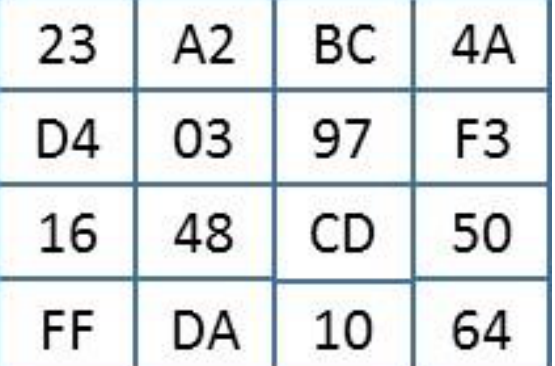
\includegraphics[width=60.69mm,height=100.68mm]{../../images/llm/page_017_img_01.png}%
\end{textblock*}

\end{document}
